\chapter{Introduction}\label{Introduction}

Our understanding of the Universe has advanced with the advancement in our 
theoretical, observational and computational abilities in the last two decades. 
While we are confident about the flatness of the Universe from CMB experiments, 
the indicative accelerating Universe from Supernovae-Ia surveys is well supported
by a cosmological constant. Finally a non-interacting dark matter is essential 
to explain the kinematics of galaxies in clusters, lightcurves of galaxies, 
gravitational lensing etc. A comprehensive model, the so-called $\Lambda$CDM,
is very successful in explaning most of the observations independently and 
combined constraints tells us that our Universe is composed of about 70$\%$
dark-energy in the form of cosmological constant $\Lambda$, about 25$\%$ non-interacting
cold dark-matter (CDM) and only 5$\%$ of the baryonic/ordinary matter. 

%------------------------------------------------------------------------------



\section{An Expanding Universe}

A stationary Universe would be boring, we have an expanding one - even better its
accelerating. The evidences are found in various probes like SNe-Ia \cite{}, 
CMB \cite{}, BAO \cite{}, galaxy clustering \cite{}, Lyman alpha \cite{} etc. 
The state-of-the-art was seeded when somebody sees something \cite{} which is 
further improved/informed by someone else \cite{}. 

Adding the so-called {\it cosmological principle} to the Einstein's field equations, 
which relates the Einstein tensor (geometrical object) to the Energy-Momentum tensor, 
derives the Friedmann equations:

\begin{equation}
\centering
\left( \dfrac{\dot{a}}{a} \right)^2 = \dfrac{8 \pi G}{3} \rho - \dfrac{Kc^2}{a^2},
\label{eqn:fe1}
\end{equation}

\begin{equation}
\centering
\left( \dfrac{\ddot{a}}{a} \right) = -\dfrac{4 \pi G}{3} \left( \rho + \dfrac{3p}{c^2} \right),
\label{eqn:fe2}
\end{equation}
\\
where, $\rho$ and $p$ are the density and pressure of the corressponding component of
the energy density of the Universe, $a$ is the scale factor for the size of the expanding
Universe normalised to unity at present ($a_0=1$).
$K$ is the curvature parameter and follows $K=0$ for a flat Universe. $G$ and $c$ are
the Gravitation constant and speed of light respectively. Related by equation \ref{eqn:fe1} 
and \ref{eqn:fe2}, the dynamics and expansion of the Universe depend on its contents. 
Combining these two equations give a third equation, also known as {\it third} Friedmann
equation:

\begin{equation}
\centering
\dot{\rho} = -3 \dfrac{\dot{a}}{a}(\rho + p).
\label{eqn:fe3}
\end{equation}

These three equations completely describe the dynamics of the Universe at all times.
The first two equations relates the matter variables ($\rho$ and $p$) to the geometric
variables ($a$ and $K$) whereas the third equation resembles the first law of 
thermodynamics for adiabatically expanding Universe, fairly approximated.

One can also relate $\rho$ and $p$ with an {\it equation of state}:

\begin{equation}
\centering
p = w \rho,
\label{eqn:eos}
\end{equation}
\\
$w$ is known as the equation of state variable for the respective component
of the energy density of Universe. For non-relativistic matter like dust $w=0$,
for photons and relativistic neutrinos $w=1/3$ whereas for a cosmological constant
$w=-1$. Analysing equation \ref{eqn:fe2}, suggests that $w<-1/3$ is essential to
have an accelerating Universe ($\ddot{a}>0$) which is the general case for the
dark-energy component with cosmological constant as a special case when $w=-1$.

Combining equation \ref{eqn:fe3} and \ref{eqn:eos} for a constant $w$, we get:

\begin{equation}
	\rho(a) = \rho a^{3(1+w)}
	\label{eqn:rho_t}
\end{equation}
\\
giving the evolution of the densities of different components driven by their 
respective equation of state. From now onwards we define $w$ to be the equation of 
state of dark-energy unless stated otherwise.

The curvature parameter $K$ in equation \ref{eqn:fe1} changes sign with the expansion 
rate, therefore $K=0$ is a limiting case. Employing equation \ref{eqn:fe1} today with
$K=0$ yields,

\begin{equation}
	\rho_{cr} \equiv \rho_0 = \dfrac{3H_0^2}{8\pi G}
\end{equation}
\\
Where, we define the expansion rate of the Universe as:
\begin{equation}
	H(t) \equiv \dfrac{\dot{a}}{a}; H_0 \equiv H(t=0) = \dot{a}(t_0)
\end{equation}
\\
where, $H_0$ is the Hubble parameter today or also referred as Hubble constant. In 
practice it is parameterized as $h$ in units of 100 km/s/Mpc.

The critical density $\rho_{cr}$ is a characteristic density of the Universe and is
used to scale the densities of various components as,

\begin{equation}
	\Omega_m \equiv \dfrac{\rho_{m0}}{\rho_{cr}};
	\Omega_r \equiv \dfrac{\rho_{r}}{\rho_{cr}};
	\Omega_{\Lambda} \equiv \dfrac{\rho_{\Lambda}}{\rho_{cr}};
	\label{eqn:Omega}
\end{equation}

Using equation \ref{eqn:Omega} and \ref{eqn:rho_t}, we can rewrite equation \ref{eqn:fe1} 
as:

\begin{equation}
	E^2(a) \equiv \dfrac{H^2(a)}{H_0^2} = \left[\dfrac{\Omega_r}{a^4}
	 + \dfrac{\Omega_m}{a^3} +
	 \Omega_{\Lambda} - \dfrac{Kc^2}{a^2H_0^2}  \right]
\end{equation}

Now it is straightforward to calculate the age of the Universe at time $t$ from the big bang
when scale factor was $a(t)$,
\begin{equation}
	H(a) = \dfrac{\dot{a}}{a} = \dfrac{1}{a} \dfrac{da}{dt},
\end{equation}
\\
which gives,
\begin{equation}
	dt = \dfrac{da}{aH(a)},
\end{equation}
\\
and therefore,
\begin{equation}
	t(a) = \int_0^a \dfrac{da^{\prime}}{a^{\prime}H(a^{\prime})}.
\end{equation}
\\
This equation gives the age of the Universe when its size was
scaled to the scale factor $a$ with respect to the present. Hence, both $t$ and
$a$ defines the epoch in the cosmic history of the Universe.

%-----------------------------------------------
\subsection{Cosmological redshift}

Consider a source at time $t$ in the cosmic history emitting light reaching us today. 
Due to the expansion of the Universe, the wavelength of the light observed 
($\lambda_{\rm obs}$) will be different (stretched or redshifted) from the 
wavelength at which it was emitted ($\lambda_{\rm emit}$) by a factor by which
the Universe is expanded during the travel time of the photons, i.e.,
\begin{equation}
	(1+z) \equiv \dfrac{\lambda_{\rm obs}}{\lambda_{\rm emit}} = \dfrac{a_{\rm obs}}{a_{\rm emit}}
\end{equation}
\\
and as conventionally we define $a_{\rm obs} = a_{\rm today} = 1$, we have,
\begin{equation}
	(1+z) = \dfrac{1}{a(t)}
\end{equation}
\\
where, $z$ is known as the cosmological redshift of the source and also describe
the epoch in the cosmic history of the Universe. Therefore, the terms scale factor 
$a$ and redshift $z$ and cosmic time $t$ will be used interchangeably 
characterizing the epoch in the cosmic history of the Universe. 


%-----------------------------------------------
\subsection{Cosmological distances}
As the Universe is expanding with cosmic time, the notion of distance to a source
is not strict and characterizes conceptually. So if we go in the frame of reference
which is expanding with the Universe, or the so-called comoving coordinates, we can
define a comoving distance ($\chi$) as the distance to the radial coordinate of a source in
an expanding Universe,

\begin{equation}
	-\mathrm{d}\chi(a) = \dfrac{c\mathrm{d}t}{a} = 
	\dfrac{c\mathrm{d}a}{a \dot{a}} = \dfrac{c\mathrm{d}a}{a^2 H(a)}
\end{equation}
\\
or,
\begin{equation}
	\mathrm{d}\chi(z) = \dfrac{\mathrm{d}z}{H(z)} 
	\Rightarrow \chi(z) = \int_0^z \dfrac{\mathrm{d}z}{H(z)}
\end{equation}
\\
$\chi(z)$ is the radial comoving distance to redshift $z$. 

Suppose one knows the size ($d$) of a source at redshift $z$ and hence measure its
distance by measuring the angle subtending to the observer ($\theta$), this distance is referred
to as angular diameter distance and define as,
\begin{equation}
	D_{\rm ang}(z) = \dfrac{d}{\theta} = a(z)\chi = \dfrac{\chi}{1+z}
\end{equation}
\\
the multiplicative factor $a(z)$ is due to the fact that the Universe was smaller by 
a factor of $a$ when the light was emitted. 

Similarly, if one measure the flux ($S$) from a source and model its luminosity ($L$), it is
possible to infer the distance to the source referred as Luminosity distance and 
given by,
\begin{equation}
	D_{\rm lum}(z) = \sqrt{\dfrac{L}{4\pi S}} = \dfrac{\chi}{a(z)} = (1+z)\chi
\end{equation}
\\
the multiplicative factor of ($1/a(z)$) is due to the redshifted photons during the
expansion of the Universe.


%------------------------------------------------------------------------------
\clearpage
\section{Structure Formation in the Universe}

An absolutely homogeneous Universe would be very easy to write mathematics for, but 
would be boring. Thanks to the inhomogeneties in the Universe, we exist. The seeds
of those homogeneties were the tiny quantum fluctuation, which in our concordance 
model, is stretched up by the {\it inflation} and transform into small density
perturbations. As a result of gravitational instability, these small perturbations 
grow and form structures at various scales following baryonic physics. 
So, the history of the  structure formation in the Universe, as described in the 
concordance model can be studied in two parts: (i) {\it Linear theory}, when
the size of the perturbation were small and higher orders terms can be ignored and 
(ii) {\it Non-linear theory}, when the size of the perturbations grows significantly
large that higher order terms cannot be ignored.

Starting from CMB and Recombination era, talk about homogeneous Universe, matter-
dominated Universe, dark-ages etc.

Hierarchical structures, observational constraints, Re-ionization.

%----------------------------------------------
\subsection{Linear theory}


We start by defining the density contrast, the relative deviation of the density
from the mean background density of the Universe,

\begin{equation}
	\delta(r,t) = \dfrac{\rho(r,t) - \bar{\rho}(t)}{\bar{\rho}(t)},
\end{equation}
\\
where, $\bar{\rho}(t)$ is the mean matter background density 
of the Universe at that epoch. 
As suggested by the tiny fluctuations in the CMB temperature anisotropy, 
the perturbations in the density field at cosmological scales during 
the early times were small. Hence, the higher powers of $\delta$ terms
can be neglected and thus the predictions of linear perturbation theory
are valid at early times.

Assuming a matter dominated Universe, which is a good approximations at the
early times, with dark-matter as the dominant component being collisionless. 
So, we can approximate the matter as a pressureless fluid which is fairly 
valid at large scales. The fluid equations for vanishing pressure are: 
(i) Continuity equation, describing the conservation of matter; (ii) Euler
equation, describing the equation of motion for the fluid and finally (iii) 
Poisson equation describing the gravitational field. Solving these three 
equations in linear regime, Fourier space and comoving coordinates will give
the so-called {\it Growth equation}:

\begin{equation}
\centering
\dfrac{\partial^2\delta}{\partial t^2} + \dfrac{2\dot{a}}{a} 
		\dfrac{\partial\delta}{\partial t}
		- \dfrac{3H_0^2 \Omega_m}{2a^3} \delta = 0
\end{equation}
\\
This equation is fair approximation at large scales, where the perturbations
are small and completely describe the distribution and evolution of perturbations. 
The equation resembles a harmonic oscillator with damping
term govern by the Hubble parameter. The solution to this equation can be 
separated in spatial and temporal part, where the temporal part gives the 
growth of the structures, $D_+(t)$, and therefore,

\begin{equation}
	\dfrac{\partial^2 D_+(t)}{\partial t^2} + 2 H(t)
		\dfrac{\partial D_+(t)}{\partial t}
		- \dfrac{3H_0^2 \Omega_m}{2a^3} D_+(t) = 0
\end{equation}
\\
$D_+(t)$ is also known as the growth factor. It describes the evolution of the
density fluctuations with cosmic time. But to model the density fluctuation 
at any time, we need to describe the initial condition. It is not possible
to predict/describe the fluctuation at any given spatial coordinate in space,
however, it is more wise to study it statistically and describe the statistical
properties of the density field. 

The simplest of the statistics is the two-point function. Suppose there is a 
completely random distribution of galaxies in the Universe without any deterministic 
force. Now, if we ask what is the probability of finding a galaxy close to another
galaxy at a distance $r_1$ and at another distance $r_2$, it must be the same. 
However, due to Gravitational force, due to which galaxies attracts each other, 
there is this excess probability to find a galaxy closer to another galaxy than
further. So say, the probablity of finding another galaxy at $r_1$ is larger than
at $r_2$ if $r1<r_2$.

This excess probability can be modelled as the two-point correlation function $C(x,y)$ and define as, 
\begin{equation}
	\langle \delta(x) \delta^{\star}(y) \rangle = C(|x-y|)
\end{equation}
\\
The two-point correlation function (2PCF) is only the function of the distance
separation between two points in the space. It is more convenient to work in 
Fourier space and hence we define the Fourier transform of the 2PCF as the 
power spectrum ($P(k)$) of the density field,

\begin{equation}
		\langle \tilde{\delta}(k) \tilde{\delta}^{\star}(k^{\prime}) \rangle = 
				(2\pi)^3 \delta_D(k-k^{\prime}) P(k)
\end{equation}
\\
$k$ is the wavevector at the corressponding scale. So, once we define the initial
power spectrum, along with the growth factor $D_+(t)$, we have a complete description
of the density field. Assuming the initial density field as a realization of Gaussian
random field, the task is not that complicated. This assumption lead to a simplified
expression for the linear power spectrum,

\begin{equation}
	P_{\rm Lin}(k) = A k^{n_s} T^2(k)
\end{equation}
\\
where, $n_s$ is known as the spectral index of the density field and $A$ is the
normalisation factor. $T(k)$ is known as the transfer function and describes
the scale weighting when the perturbation at those scales enters the horizon
and becomes important. 

So, as we already know that the evolution of linear perturbation grows 
proportional to the growth factor, we can thus write,

\begin{equation}
	P_{\rm Lin}(k,z) = P_{\rm Lin}(k) D_+(z)
\end{equation}

The shape of the linear power spectrum is determined by the parameter $n_s$ and 
transfer function, however, there is a different form of normalisation in 
practice such that if one counts galaxies in sphere of radius 8 $Mpc/h$, then
the average relative error is close to unity. 

So, we define the variance of the smoothed density field as,

\begin{equation}
	\sigma^2(R) = \int \dfrac{d^3k}{(2\pi)^3} |\tilde{W}(k,R)|^2 P(k)
\end{equation}
\\
where, $\tilde{W}(k,R)$ is the Fourier transform of the tophat function smoothed 
at scale $R$ and given by,

\begin{equation}
	\tilde{W}(k,R) = 3\dfrac{\sin(kR) - kR \cos(kR)}{(kR)^3}
\end{equation}
\\
and therefore we have,

\begin{equation}
	\sigma^2(8 Mpc/h) \equiv \sigma_8^2 \approx 1
\end{equation}
\\
$\sigma_8$ is the parametrisation in practice to normalize the power
spectrum. 

\subsection{Zeldovich approximation}

In Lagrangian perturbation theory (LPT) \cite{} at large scales where matter is
well approximated as fluid, one can write the position each element of the fluid as
\begin{equation}
	x(q,t) = q + \Psi(q,t)
\end{equation}
\\
where, $q$ is the initial position of the element and $\Psi(q,t)$ is the Lagrangian
displacement field. $q$ and $\Psi(q,t)$ together completely describe the motion
of the cosmological fluid at any time. In LPT, one can try to find the solution 
perturbatively,

\begin{equation}
	\Psi(q,t) = \Psi^{(1)}(q,t)+\Psi^{(2)}(q,t)+\Psi^{(3)}(q,t)+\dots
\end{equation}

The first order solution ($\Psi^{(1)}(q,t)$) is the Zeldovich approximation (ZA). It
is an intuitive way to understand the filamentary structures in the cosmic web 
and understanding of non-linear structure formation. As only first order term
is considered in LPT, the approach is quasi-linear in nature.

There are particularly two advantages of using ZA instead of linear theory:

\begin{itemize}
	\item First, it is easy to include the redshift space distortions in this formalism,
	\item Second, Even though ZA is in a sense linear, it provides non-linear smearing
	to the BAO feature to the amount that matches the simulations very well. 
\end{itemize}

The Zeldovich power spectrum is given by (see e.g. \cite{})
\begin{align}
(2\pi)^3&\delta^D (k)+P(k)=\int d^3 q ~e^{-i\VEC{q}\cdot\VEC{k}}\nonumber\\
&\times\exp\left[-\frac{1}{2}k_ik_jA_{ij}(\VEC{q}))\right],
\label{eq:PSwithAW}
\end{align}
where 
\begin{equation}
A_{ij}(\VEC{q})=X(q)\delta^K_{ij}+Y(q)\hat{q}_i\hat{q}_j,
\end{equation}
and
\begin{align}
  X(q) =& \int_0^\infty \frac{dk}{2\pi^2} P_L(k)
  \left[\frac{2}{3} - 2 \frac{j_1(kq)}{kq}\right] , \\
  Y(q) =& \int_0^\infty \frac{dk}{2\pi^2} P_L(k)
  \left[-2 j_0(kq) + 6 \frac{j_1(kq)}{kq}\right] .
  \label{eq:XYex}
\end{align}
Here $P_L(k)$ is the linear power spectrum and $j_n$ is the spherical Bessel function of order $n$. 

%----------------------------------------------
\subsection{Non-Linear theory}

At late times or at small scales, the approximation $\delta << 1$ breaks. So, the analytical
description becomes difficult/impossible for the structure formation. The solution then would 
be to rely on simulations, higher order perturbation theory, physical approximations to the
distribution of the matter in the Universe or semi-analytic approaches. Analogous to these
approaches, there are various estimators for the power spectrum of the matter density field,
here we discuss two of them: N-body simulations (Numerical solution) and the halo model (
Analytic approximatoin).

\subsubsection{N-body simualtions}

With advancement in the compuatational power in the last decade, it is now possible to
simulate the Universe at cosmological volumes to high accuracy up to the scales where
only gravity is important in structure formation. These scales are highly non-linear and
very difficult to describe by higher order perturbation theories etc. An N-body simulation
characterizes to simulate a Universe consists of only dark-matter (and no baryons) that 
interacts only gravitationally. Such a simulation is useful in studying the
structure formation at scales large enough that baryonic processes are not 
important and small enough that the clustering processes are non-linear and difficult
to describe analytically. 

It is not possible (or at least very expensive) to simulate a volume equivalent to the
observable Universe, but only a part of it. Assuming that the Universe is homogeneous
at cosmological scales (or the scales of the largest structures BAO), the simulation
volume must at least include these structures. So a cube with side length nearly 200 Mpc/h
is needed to simulate a true representative of the Universe. Larger volumes are needed
for various other purposes, e.g., covariance matrix (to be discussed in section \ref{}).

One very important ingredient of a simulation is the initial conditions which are
set to very high redshift and let the particles evolve with gravity up to redshift zero. 
The best way to set the initial condition is to put all the particles in a uniform 3D grid
and then displace each particle with a displacement field to match the initial power 
spectrum (linear). 

Another important aspect of a simulation is its resolution. This depends on the number 
particles or the mass of each dark-matter particle (at least one of them is free parameter 
to fix at the beginning). Smaller is the mass of the individual dark-matter particle, 
larger will be the total number of particles in order to match the critical density of 
the Universe today and therefore, one can resolve smaller scale structures. However, 
there is always a trade-off between large volumes and higher resolutions. 

Some examples of top simulations here...Emulator, Skillman, Aurel's simulations etc. 



\subsubsection{The halo model}

The halo model is one of the more successful analytic and physical framework to describe
the clustering and growth of structures in the Universe. In this framework, all the matter
in the Universe is assumed to be in the form of spherical halos whose radius are defined by a 
density threshold, usually uses as the 200 times the mean matter density of the Universe 
(e.g., $R_{200}$). The  distribution of halos are assumed to follow a radial density 
profile, which depends on the mass of the halos, truncated at $R_{200}$ or at virial 
radius ($R_{\rm vir}$).

The assumptions of the halo model are invalid in details but are well approximated and 
hence the estimators for the matter power spectrum are well in agreement 
(nearly 20$\%$ at non-linear scales)
to the more accurate simulations. However, due to these invalid approximations, it is not
possible to achieve higher accuracy, like sub-percent, with this estimator. 

There are particularly four ingredients to model the power spectrum in halo model framework:

\begin{itemize}
	\item Linear power spectrum.

	\item Radial density profile of the halos. Usually for dark-matter only Universe, the so-called
			Navarro-Frenk-White (NFW) is used as a Universal profile completely characterized by the
			mass (or concentration) of the halo,
			\begin{equation}
				\rho(r) = \dfrac{\rho_s}{(r/r_s)(1+r/r_s)^2}
			\end{equation}
			\\
			where, $r_s$ and $\rho_s$ are the scale radius and characteristic density at scale radius
			respectively. Here we define the concentration parameter of the halo as,

	\item Mass function ($f(M)$): a functional form defining the number of halos as a function of halo
			mass. 

	\item Halo bias: As the halos are biased tracers of the matter, one important ingredient is 
			the description of the bias.  
\end{itemize}

Once we know these four ingredients, it is very straightforward to model the power spectrum. For 
more details see chapter \ref{}

\subsection{Baryonic contributions}
It is relatively easy to model and describe the clustering of matter that interacts with only 
one force (gravity) aka dark-matter. But we exist and not made up of dark-matter, instead by the
ordinary matter we know as baryons which interacts other than gravity too and exhibit pressure. 
Even the Universe with baryons and dark-matter would behave very similar at large scales,
but at small scales where the baryonic processes are important, dark-matter only Universe is
not a good description. 

To model the structure formation with baryons, is rather a messy task. Analytic calculations
can be very complicated and not-reliable. However, simulations are better ways. One can always
put baryonic matter along with dark matter in the simulations and evolve governing gravity and
baryonic processes which are known to be important. Some of the processes are described below,

\begin{itemize}
	\item Star formation
	\item Feedback processes
	\item Radiative transfer
	\item Adiabatic contraction/expansion
\end{itemize}

When there is very little understanding of start formation processes, other processes can be 
modelled with some approximations. But carrying out these calculations in big cosmological 
volumes are very expensive and may still be out of the reach to the current computational 
abilities. 

The other way is to include the baryonic processes is to perturb the density profile 
of the halos with baryonic processes and model with the halo model. This approach can 
be calibrated with simulations or observations but still remain analytical with some 
free parameters to be measured by data directly. For a similar approach see chapter \ref{}



\subsection{Covariance matrix of matter power spectrum}
As the 2PCF and power spectrum are statistical quantities, there is a statistical limit
to which it can be measured in cosmological surveys or simulations. This limit is expressed
as the covariance matrix. 

The full covariance matrix of the matter power spectrum consist of three broad parts:

\begin{itemize}
	\item Gaussian part:
	\item Non-Gaussian part:
	\item Super-sample variance: 
\end{itemize}





%------------------------------------------------------------------------------
%------------------------------------------------------------------------------
\clearpage
\section{Probes of Cosmology}

Starting general ideas and all possible probes of cosmology with preferences.
\begin{itemize}
	\item CMB
	\item BAO
	\item Supernovae-Ia
	\item Galaxy cluster
	\item Sunyaev Zeldovich effect
	\item Lyman alpha forest
	\item 21cm cosmology
	\item Redshift space distortions
	\item Gravitational lensing
\end{itemize}


%------------------------------------------------------------------------------

\subsection{Gravitational Lensing}
The bending of light from a distant source due to the gravitational field of the
intervening matter is known as
the gravitational lensing (or lensing henceforth). It is a powerful technique to 
obtain information about the intervening matter (or the lens from now). There are
various observables due to this phenomenon like multiple-images of the source, time 
delays amongst the multiple-images, shape distortion of the source, change in brightness
of the source etc. Each of these observables can be utilised to infer or model various
aspects: from the mass distribution of the lens to cosmology. As lensing phenomenon depends 
on the total mass of the lens and not on its nature (dark-matter or baryonic), it is
so far the most unbiased technique to probe the distribution of matter in the Universe
and to do cosmolgoy.

\begin{figure}
	\centering
	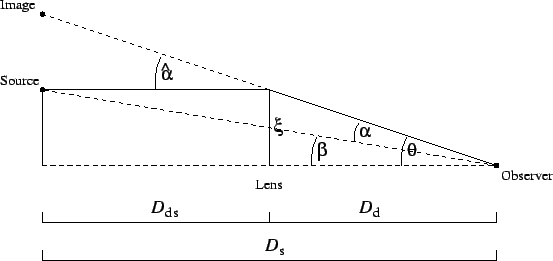
\includegraphics[width=0.7\textwidth]{figures/lens_geometry.png}
	\caption{}
	\label{fig:lens}
\end{figure}

Consider figure \ref{fig:lens}: a ray of light from a source, at a distance $D_s$ from
the observer, deflected due to the lens, at a distance $D_d$ from the observer,  by an 
angle $\hat{\alpha}$ and seen
by the observer at an angle $\theta$ from the lens. If there were no lens, it would have
been observed at $\beta$. Employing small angles approximations, 

\begin{equation}
	\beta  = \theta  - \dfrac{D_{ds}}{D_s} \hat{\alpha}(\xi) \equiv \theta - \alpha(\xi)
	\label{eqn:lens}
\end{equation}
\\
where, $\alpha$ is the scaled deflection angle with respect to the center of the 
lens to the observed position of the source image and $\xi$ is the impact parameter
of the image on the lensplane. The equation \ref{eqn:lens} is known
as the lens equation. The equation describes the true position of the source at $\beta$ to
be seen at $\theta$ due to the lens which is deflecting the light rays by an angle $\alpha$.
If this equation has more than one solution, there will be multiple images of the source. 

The deflection angle $\hat{\alpha}$ depends on the impact parameter as well as the 
mass/density distribution of the lens. For a spherically symmetric lens, general relativity
predicts,
\begin{equation}
	\hat{\alpha} = \dfrac{4GM}{c^2 \xi}
\end{equation}
\\
which is twice the value predicted by Newtonian gravity. For more complex lenses, the 
relation between the deflection angle, impact parameter (or $\theta$) and the mass
distribution of the lens can be obtained under the so-called geometrically thin lens
approximation as,

\begin{equation}
	\alpha(\theta) = \dfrac{1}{\pi} \int d^2\theta^{\prime}
						\kappa(\theta^{\prime})
						\dfrac{\theta-\theta^{\prime}}{|\theta-\theta^{\prime}|^2}
\end{equation}
\\
where, $\kappa(\theta)$ is the surface mass density in the units of a critical 
density $\Sigma_{\rm cr}$ defined as,

\begin{equation}
	\kappa(\theta) \equiv \dfrac{\Sigma(\theta)}{\Sigma_{\rm cr}}; 
	\Sigma_{\rm cr} = \dfrac{c^2}{4\pi G} \dfrac{D_s}{D_d D_{ds}}.
\end{equation}

The critical density completely depends on the geometry of the system. For generating
multiple images, $\kappa>1$ and hence the critical density is a characteristic 
surface mass density in order to produce extra images for some values of $\theta$.
Therefore, critical density is also characteristic to differentiate between region
of strong and weak lensing, which are described in more details below.

%----------------------------------------------
\subsubsection{Strong Gravitational Lensing}




%----------------------------------------------
\subsubsection{Weak Gravitational Lensing}
%----------------------------------------------
\subsubsection{Microlensing}

%------------------------------------------------------------------------------
%------------------------------------------------------------------------------
\clearpage
\section{Essential statistics for cosmology}
There are two broad schools in statistics Frequentist and Bayesian. Frequentists believe
that parameters are all fixed and unknown constants in the model whereas Bayesians
believe that parameters are random variables that has a given distribution, and other probability
statements can be made about them. According to Frequentists, there are TRUE
population parameters that are unknown and can only be estimated by the data whereas,
Bayesians believe that only data are real; the population parameters are an abstraction, and
as such some values are more believable than others based on the data and on prior beliefs.
In other words, Bayesian defines the probability as the degree of belief where Frequentists
termed it as frequency of occurrence in a set of trials. 

\subsection{Statistical Inference}



\subsection{MCMC and Fisher}
\subsection{Genetic algorithm}

%------------------------------------------------------------------------------
%------------------------------------------------------------------------------
\clearpage
\section{Motivation}

Here I would like to give a comprehensive summary of this work.

\subsection{Challenges}
\subsection{What are we trying to achieve}
\subsection{A unified picture}

%------------------------------------------------------------------------------

\clearpage
\cite{2014MNRAS.440.2290M}

\cite{2014MNRAS.439.2651M}

\cite{2014A&A...567A..65B}

\cite{2014MNRAS.445.3382M}

\cite{2014arXiv1410.6826M}

\cite{2015PASJ...67...21M}

\cite{2015arXiv150403388M}





